\section{ПРОЕКТИРОВАНИЕ}
    \subsection{Концептуальная модель обработки сообщений}
    Главной целью при разработке новой архитектуры чат-бот ставилась возможность
    разбиение процесса обработки на основные этапы, которые можно было бы
    распределить между независимыми классами, с единственной ответственностью и
    высоким потенциалом переиспользования.
    Процесс обработки сообщения можно разделить на следующие этапы:
    \begin{enumerate}
        \item Получение сообщения через интерфейс (IMAP, LongPoll ВКонтакте, 
        telegram-api, http-POST)
        \item Извлечение необходимых полей из инородной структуры данных и 
        преобразование в объект-сообщение внутреннего типа
        \item Классификация сообщения
        \item Формирование ответов на сообщение
        \item Отправка ответов обратно через интерфейс библиотеки пользователю
        \item Сохранение всех сообщений в базу
        \item Выполнение дополнительных действий (запрос обратной связи от
        пользователя, логгирование и прочее)
    \end{enumerate}

    Таким образом, за каждый из этапов обработки сообщения отвечать будет свой 
    отдельный объект, притом, на этапе 3 и 4 абсолютно не важно, по какому 
    каналу было получено сообщение, равно как на этапе 5, 6 и 7. Этапы 1, 2 и 5, 
    наоборот, направлены исключительно на адаптацию к внешним API и библиотекам.
    Для их реализации будет применен паттерн "Адаптер". Для реализации этапов
    6 и 7 будет использован паттерн "Наблюдатель" - таким образом,
    заинтересованные объекты-подписчики будут уведомлены о новом сообщении в чатах.
    \cite{design.patterns}
    
    \subsection{Описание участников обработки сообщений}
    \subsubsection{ApiWorker}
    Класс-адаптер ответственный за первый этап -- \inlinecode{ApiWorker}.
    Его ответственность -- постоянная обработка входящих сообщений от 
    пользователя и исходящих сообщений от оператора и бота, используя библиотеки
    для работы с каналами. Обладает одним методом, который запускает процесс 
    получения новых сообщений. Его код представлен на рисунке 1.
    \begin{figure}[H]
        \centering
        \lstinputlisting[language=Python]{snippets/api_worker.py}
        \caption{Код класса ApiWorker}
        \label{fig:api_worker}
    \end{figure}


    \subsubsection{ApiWrapper}
    Ещё один класс-адаптер, ответственный за превращение полученного сообщения 
    во объект-контейнер MessageData, обратное превращение перед отправкой
    сообщения пользователю и непосредственную отправку.
    Его интерфейс выглядит так как показано на рисунке 2:
    \begin{figure}[H]
        \centering
        \lstinputlisting[language=Python]{snippets/api_wrapper.py}
        \caption{Код класса ApiWrapper}
        \label{fig:api_wrapper}
    \end{figure}
    
    Метод \inlinecode{send_answers} отправляет все ответы из списка, дополняя их
    необходимой информацией от сервера текущего канала. 
    Метод \inlinecode{send_message} отправляет одно отельное сообщения по текущему каналу,
    возвращает то же сообщение, но дополненное информацией от сервера: реальным временем
    отправки, идентификатором, который сервер канала обозначил это сообщение и так далее.


    \subsubsection{MessageHandler}
    Все действия между получением сообщения в \inlinecode{ApiWorker.run} и отправкой ответов
    в \inlinecode{ApiWrapper.send_answers} и сохранением в базу будет скрывать в себе метод
    \inlinecode{MessageHandler.handle}. Для входящих сообщений от пользователя обрабатывать
    сообщения будет IncomingHandler, для исходящих от оператора и бота -- OutgoingHandler.
    Интерфейс класса MessageHandler представлен на рисунке 3.
    \begin{figure}[H]
        \centering
        \lstinputlisting[language=Python]{snippets/message_handler.py}
        \caption{Код класса MessageHandler}
        \label{fig:message_handler}
    \end{figure}

    Метод \inlinecode{MessageHandler.notify} здесь исполняет отправку всех уведомлений,
    которые были переданы ему от объекта класса \inlinecode{ApiWorker}.

    Обработчик входящих сообщений, \inlinecode{IncomingHandler},
    также должен вырабатывать ответ к входящему сообщению. 
    Эту задачу он делегирует другому классу -- \inlinecode{Scenarist}. 
    Дополнительно \inlinecode{IncomingHandler} может исполнять некоторые
    действия, в зависимости от выбранного сценария.
    Общий вид класса представлен на рисунке 4.
    \begin{figure}[H]
        \centering
        \lstinputlisting[language=Python]{snippets/incoming_handler.py}
        \caption{Код класса IncomingHandler}
        \label{fig:incoming_handler}
    \end{figure}

    Все участники получения и обработки входящих и исходящих сообщений, а также
    отправке ответов на последние, изображены на рисунке 5.
    \begin{figure}[H]
        \centering
        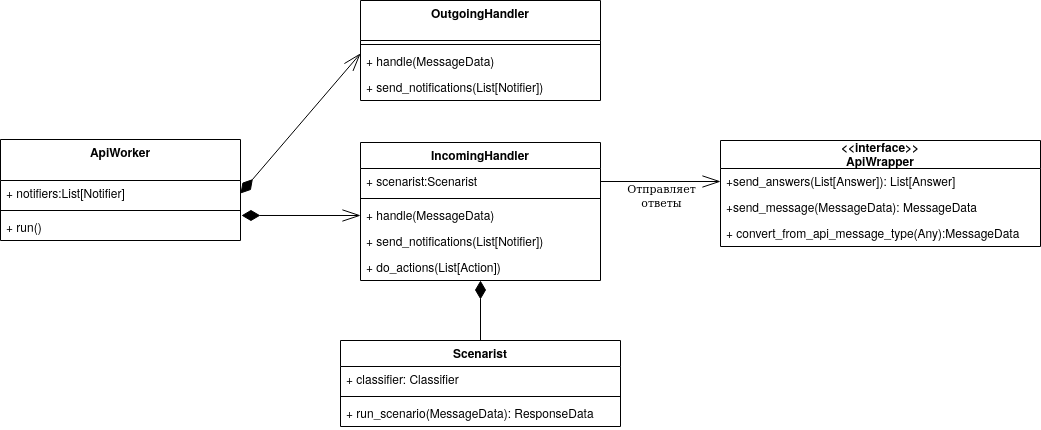
\includegraphics[width=\linewidth]{static/ClassDiagram_ioprocess.png}
        \caption{Диаграмма классов -- система обработки сообщений}
        \label{fig:class-diagram-ioprocess}
    \end{figure}


    \subsubsection{Notifier}
    Если событие, произошедшее во время работы объекта ApiWorker необходимо
    зарегистрировать, то для этого будет использован один из классов,
    реализующих интерфейс Notifier.
    Схема уведомлений реализована в соответствии с паттерном "издатель-подписчик".
    Каждый ApiWorker обладает набором Notifier-подписчиков, каждому из которых
    отправляется уведомление о событии \inlinecode{Notifier.notify}.
    Уведомления могут понадобиться для создания записи в базе о новых сообщениях,
    или для отправки логов работы в мессенджер разработчика или заказчика.
    Диаграмма классов, связанных с отправкой уведомлений изображена на рисунке 6.
    \begin{figure}[H]
        \centering
        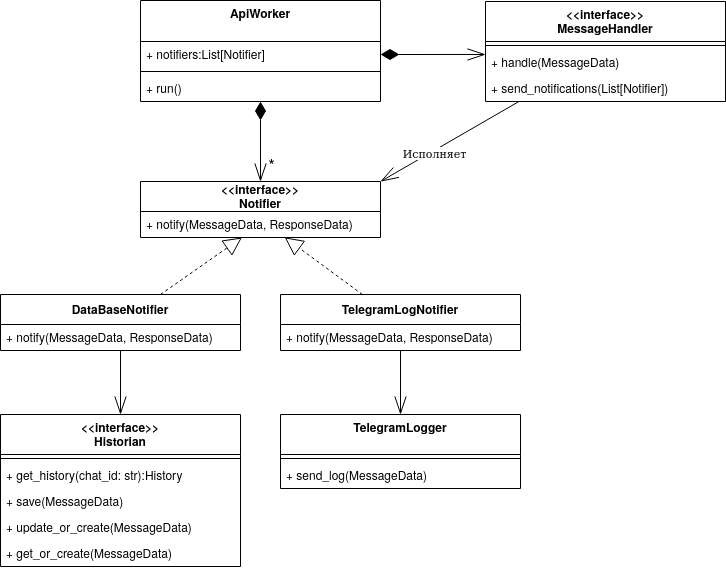
\includegraphics[width=0.9\linewidth]{static/ClassDiagram_notifiers.png}
        \caption{Диаграмма классов -- уведомления}
        \label{fig:class-diagram-notifiers}
    \end{figure}


    \subsubsection{Сценарист}
    Scenarist -- класс сценариста, обладает только одним методом:\\
    \inlinecode{Scenarist.run_scenario}, который должен
    выработать нужную реакцию (ResponseData) на входящее сообщение с
    набором нужных ответов (Answer) и действий (Action).

    Задачу предсказания сценарист делегирует классификатору (Classifier),
    обладающему единственным методом \inlinecode{Classifier.predict}, который
    возвращает объект Prediction с набором меток обнаруженных в тексте сообщения
    классов. По этим меткам и будет составлена ResponseData внутри сценариста.

    Сам классификатор использует объект модели, интерфейс которой описан в
    \inlinecode{AbstractModel} -- модель получает на вход метода
    \inlinecode{AbstractModel.predict_proba} текстовое сообщение и возвращает
    вероятности принадлежности сообщения к одному из множества классов,
    описанных в поле \inlinecode{AbstractModel.labels} объекта. Модель может
    иметь одну из двух реализаций: реальная модель -- \inlinecode{RealModel},
    или оболочка для удаленного доступа к модели \inlinecode{RemoteModel}.
    В случае с удаленной моделью, классификация осуществляется через вызов
    удаленной процедуры, зарегистрированной с задаче Celery.
    Это будет заложено для того, чтобы тяжеловесную модель можно было использовать
    из легковесных процессов Django.

    Увидеть зависимости сущностей, связанных с выработке сценария, можно увидеть
    на рисунке 7.
    \begin{figure}[H]
        \centering
        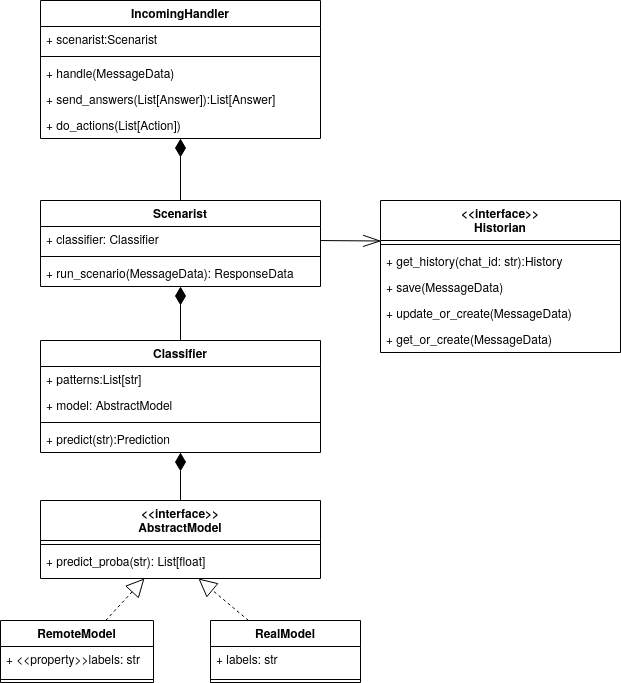
\includegraphics[width=0.8\linewidth]{static/ClassDiagram_classifier.png}
        \caption{Диаграмма классов -- диалоговая система}
        \label{fig:class-diagram-classifier}
    \end{figure}


    \subsubsection{Историк}
    Для ведения длительного диалога с пользователем сценаристу требуется история
    диалога. Для ведения и доступа к истории чатов будет использоваться интерфейс
    "Историк" - \inlinecode{Historian}. Он не подразумевает конкретный вид хранения
    диалога - это может быть реляционная или нереляционная база данных,
    оперативная память или файловая система.
    
    Работа с базой данных через объектно-реляционную модель будет инкапсулирована
    в классе DataBaseProvider, которые реализует все необходимые интерфейсные
    методы историка. Диаграмму классов, связанных с хранением и получением
    истории, можно увидеть на рисунке 8.
    \begin{figure}[H]
        \centering

        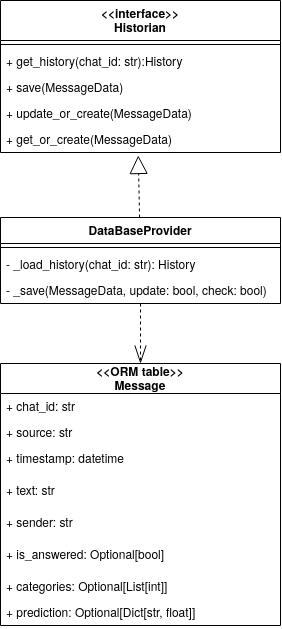
\includegraphics[width=0.3\linewidth]{static/ClassDiagram_dbprovider.png}
        \caption{Диаграмма классов -- система историка}
        \label{fig:class-diagram-dbprovider}
    \end{figure}

    \newpage
    \subsubsection{Типы данных}
    Также для обмена артефактами будут введены собственные типы данных.
    Описание их структуры и взаимодействия приведены на диаграмме классов ниже
    на рисунке 9.
    \begin{figure}[H]
        \centering
        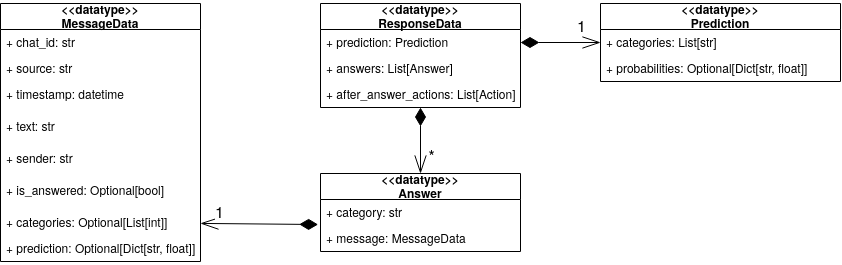
\includegraphics[width=\linewidth]{static/ClassDiagram_datatypes.png}
        \caption{Диаграмма классов -- собственные типы данных}
        \label{fig:class-diagram-datatypes}
    \end{figure}

    \subsection*{Вывод по главе 2}
    В этой главе мы сформулировали основную концепцию нашей будущей системы, 
    описали основные её сущности и способы их взаимодействия. Мы в коде описали 
    сигнатуры публичных методов её базовых классов.
    Мы также наглядно изобразили сущности и процессы системы на диаграммах классов.
    Теперь, мы можем приступать к их реализации в каждом конкретном канале.
